\chapter*{Algoritmusok}
\addcontentsline{toc}{section}{Az alkalmazás alapfunkciói}
\spacing{1.5}

A alábbi fejezetben azokrók az fraktál generáló algoritmusokról lesz szó, amelyeket a webalkalmazás részeként leimplementáltam. Minden algoritmusról egy először rövid ismertetőt írok, majd bemutatom az implementáció menetét.
\section{Sierpiński-háromszög}
A Wacław Sierpinski lengyel matematikus által megtalált fraktál úgy áll elő, hogy egy szabályos háromszögből elhagyjuk az oldalfelező pontok összekötésével nyert belső háromszöget, majd az így maradt három háromszögre rekurzívan alkalmazzuk ugyanezt az eljárást.
Hausdorff-dimenziója log(3)/log(2) ≈ 1,585.
A Sierpiński-háromszög konstrukciójához többnyire egyenlő oldalú háromszöget választanak. Ez azonban nem kötelező, bármely háromszögből lehet Sierpiński-háromszöget készíteni.
A Sierpiński-háromszög konstrukciójának lépései:
\begin{itemize}
\item Rajzolj három pontot, melyek a háromszöget határolják be, mindegyik pont a háromszög egy csúcsa
\item Rajzolj egy pontot egy tetszőleges helyre, ez lesz a kezdőpont
\item Válaszd ki a háromszög egyik csúcsát valamilyen véletlenszerű módon, majd a választott csúcsot és a kezdőpontot összekötő képzeletbeli vonal közepére rajzolj be egy újabb pontot, ez lesz az új kezdőpont
\item Ismételd ezeket a lépéseket
\end{itemize}
\begin{figure}[!ht]
\begin{center}
	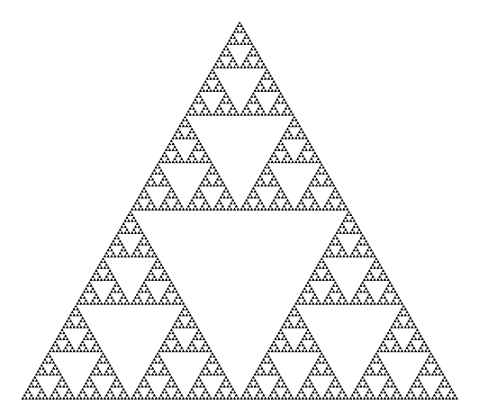
\includegraphics[width=0.5\textwidth]{SierpinskiTriangle}
	\caption[labelInTOC]{Sierpinszki háromszög}
\end{center}
\end{figure}
Minden lépésben a keletkező kis háromszögek oldalhossza megfeleződik, és területük a negyedére csökken, miközben a középső háromszög eltűnik.
\subsection{Implementáció}
A Sierpinszki-háromszög implementációjához, először egy segédosztályt írtam, mint ahogy a többi algoritmus nagy részének implementációja is segédosztályok segítségével valósult meg. Ez a segédosztály a Point osztály, mivel a Sierpinszki háromszöget az algoritmus pontok segítségével rajzolja ki. Itt definiálva vannak a pontokhoz tartozó adattagok, ez ebben az esetben egy vektor, ahol tárolódik a pont x és y pozíciója a vászon koordináta rendszerében, valamint egy draw függvény, ami kirajzolja az adott pontot. A Point osztály kódja így néz ki:
\begin{center}
\begin{tabular}{c}
\begin{lstlisting}
export class Point {
	public point: p5.Vector;
	
	constructor(point: p5.Vector) {
		this.point = point;
	}
	
	draw(p: any): void {
		p.point(this.point.x, this.point.y);
	}
}
\end{lstlisting}
\end{tabular}
\end{center}
Az implementáció többi része a fő osztályban történt meg, ami a SierpinskiTriangleConfigurable osztály. Itt többek között definiálva vannak az algoritmus konfigurációs lehetőségei is, amelyek a következők:
\begin{itemize}
	\item Gyorsaság
	\item Pontvastagság
	\item Véletlenszerű pontvastagság
	\item Pontok közötti távolság
	\item Fixált kezdőpontok
	\item Háromszög részeinek kijelölése
	\item Szín
	\item Szivárvány mód
\end{itemize}
Minden algoritmus rendelkezik egy setup és egy draw függvénnyel, amelyek a p5 könyvtárhoz tartoznak, és megvalósításuk elengedhetetlen a vászonra való rajzoláshoz. A draw függvény minden képpontfrissítéskor lefut, a setup viszont csak egyszer, mielőtt a rajzolás elkezdődne. Itt állítódnak be azok a paraméterek amelyekkel a rajzolást elkezdjük, például pontvastagság, vonalvastagság, szín, képfrissítési ráta, valamint itt jön létre a vászon objektum. Maga a rajzolás a draw függvényben történik. A SierpinszkiTriangleConfigurable osztály setup és draw függvényei így néznek ki:
\begin{center}
\begin{tabular}{c}
\begin{lstlisting}
p.draw = () => {
	this.setConfigurables(p);
	
	if (this.play) {
		let rand = p.floor(p.random(3));
		if(this.randomStrokeWeight) {
			p.strokeWeight(p.random(0, 10));
		}
	
		if(this.rainbowMode) {
			let h = p.map(p.floor(p.random(this.list.length)), 0, this.list.length, 0, 360);
			p.stroke(h, 255, 255);
		}
		else if (this.customColors && rand == 0) {
			p.stroke(this.color1);
		} 
		else if (this.customColors && rand == 1) {
			p.stroke(this.color2);
		} 
		else if (this.customColors && rand == 2) {
			p.stroke(this.color3);
		} 
	
		let newPoint = p5.Vector.lerp(this.points[rand], 
			this.refPoint, 
			this.lerpValue);
		p.point(newPoint.x, newPoint.y);
		this.refPoint = newPoint;
		
		this.list.push(new Point(newPoint));
		this.rollBackList$.next(this.list);
	}
}	
\end{lstlisting}
\end{tabular}
\end{center}
Ez egy lerövidített kód, mivel az eredeti túl hosszú, így megpróbáltam csak a lényeget szemléltetni. Látható hogy a rajzolás a különböző feltételekhez van kötve, amelyek a konfigurációktól függnek, mint például a véletlenszerű pontvastagság és a szivárvány mód. Továbbá látható, hogy a függvény csak akkor fog rajzolni, ha az algoritmus futása éppen nem szünetel. A points tömb tárolja a három pontot, amelyek a háromszöget határolják be, a refPoint változó pedig azt a pontot, amelytől a háromszög egy véletlenszerűen választott csúcsáig számítódik az a félút, ahová az új pont kerül. A véletlenszerű csúcsot a függvény a p5 random metódusa segítségével választja ki. A félút a p5 könvytár beépített lerp függvényével számolódik ki. Az refPoint változó minden új pont rajzolása esetén értékül kapja ezt az új pontot. A rollBackList\$ változó a draw függvény minden lefutása után, pontosabban minden új pont kirajzolása után, egy új értéket emittál, ezzel beállítva a visszatekerő csúszka hosszát.
\section{Sierpinski-szőnyeg}
A Sierpiński-szőnyeg szintén Wacław Sierpiński lengyel matematikus által megtalált fraktál, amely úgy áll elő, hogy egy négyzetet oldalai harmadolásával kilenc kisebb négyzetre bontunk, a középsőt elhagyjuk, és a maradék nyolcon elvégezzük ugyanezt az eljárást (vagyis azoknak is elhagyjuk a közepét), majd az így maradt 8×8 kisebb négyzeten is, stb. Az eredményül kapott alakzat területe nulla, kerülete végtelen nagy. Hausdorff-dimenziója log 8/log 3 ≈ 1,8928.
A Sierpinski-szőnyeg konstrukciójának lépései:
\begin{itemize}
	\item Vegyünk egy négyzetet
	\item Osszuk fel minden oldalát három részre
	\item A kijelölt pontokat összekötve osszuk fel a négyzetet kilenc kis négyzetre
	\item Töröljük el a középső négyzetet
	\item Ismételjük az előző lépéseket minden kis négyzetre.
\end{itemize}
Ezzel az eljárással a négyzet egyre inkább kiürül. Végtelenszer megismételve a Sierpiński-szőnyeg marad.
\begin{figure}[!ht]
	\begin{center}
		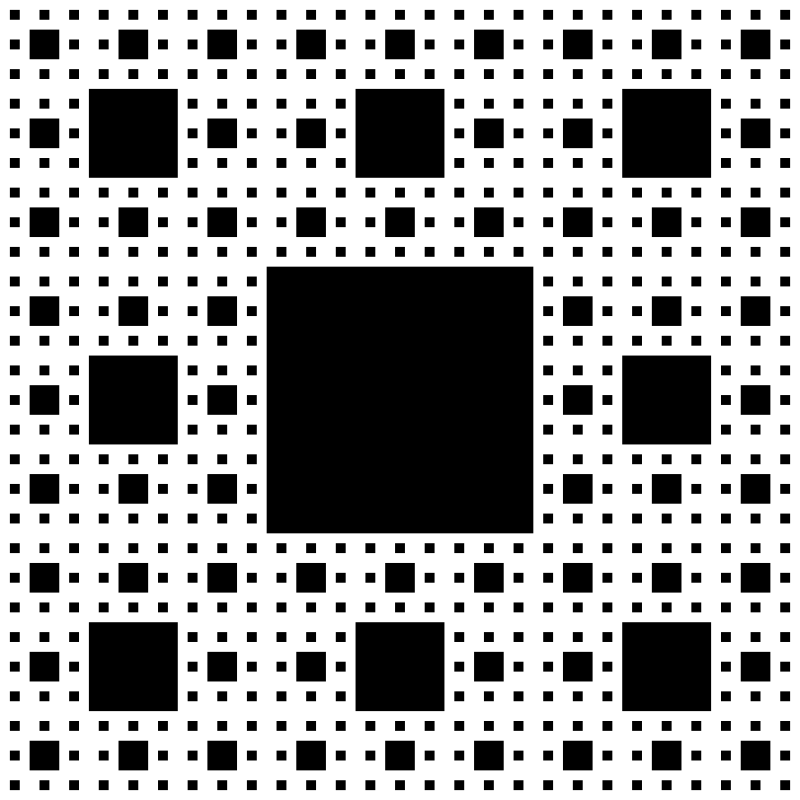
\includegraphics[width=0.5\textwidth]{SierpinskiCarpet}
		\caption[labelInTOC]{A Sierpinski-szőnyeg 4. iterációja}
	\end{center}
\end{figure}
\subsection{Implementáció}
Az implementációt, a Sierpinszki-háromszöghöz hasonlóan, itt is egy segédosztály megírásával kezdtem. Ez a segédosztály a Rectangle osztály. A segédosztály adattagként tárolja az adott négyzet középpontját, ami egy vektor objektum, és méretét. Mivel ennek a forráskódja hosszú, így csak azt a függvényt szemléltetem, amely a kilencedelést végzi. Ez az alábbi módon néz ki:
\begin{lstlisting}
divide(): Rectangle[] {
	let rectangles = [];
	
	rectangles.push(new Rectangle(
		new p5.Vector(this.center.x - this.size, this.center.y), 
		this.size / 3));
	rectangles.push(new Rectangle(
		new p5.Vector(this.center.x - this.size, this.center.y + this.size), 
		this.size / 3));
	rectangles.push(new Rectangle(
		new p5.Vector(this.center.x - this.size, this.center.y - this.size), 
		this.size / 3));
	rectangles.push(new Rectangle(
		new p5.Vector(this.center.x + this.size, this.center.y), 
		this.size / 3));
	rectangles.push(new Rectangle(
		new p5.Vector(this.center.x + this.size, this.center.y + this.size), 
		this.size / 3));
	rectangles.push(new Rectangle(
		new p5.Vector(this.center.x + this.size, this.center.y - this.size), 
		this.size / 3));
	rectangles.push(new Rectangle(
		new p5.Vector(this.center.x, this.center.y + this.size), this.size / 3));
	rectangles.push(new Rectangle(
		new p5.Vector(this.center.x, this.center.y - this.size), 
		this.size / 3));
	
	return rectangles;
}
\end{lstlisting}
Ez a függvény mindig egy négyzetre van meghívva, így az ő kilenced részét osztja fel további kilenc részre. Az algoritmus egy kezdő négyzettel indul, ami a vászon közepén helyezkedik el, így az algoritmus első iterációjában erre a négyzetre van meghívva a divide függvény. Az algoritmus konfigurációs lehetőségei a következők:
\begin{itemize}
	\item Gyorsaság
	\item Kezdő négyzet mérete
	\item Szín 
	\item Szivárvány mód
\end{itemize}
Ez az algoritmus konfigurációs lehetőségek terén nem olyan színes mint például a Sierpinszki-háromszög. Ez annak köszönhető, hogy egyszerűen nincs annyi állítható paraméter, mint az említett fraktál algoritmus esetén. A kevés konfigurációs lehetőség miatt a draw függvény is jóval egyszerűbb, mint a Sierpinszki-háromszög esetén.
\begin{lstlisting}
p.draw = () => {
	this.setConfigurables(p);

	if (this.play) {
		let newRectangles: Rectangle[] = [];
		
		for (let i = this.iter; i < this.list.length; i++) {
			if(this.rainbowMode) {
				let h = p.map(i, this.iter, this.list.length, 0, 360);
				p.fill(h, 255, 255);
			}
			this.list[i].draw(p);
			newRectangles = newRectangles.concat(this.list[i].divide());
		}
		
		this.rollBackList$.next(this.list);
		this.iter = this.list.length;
		this.list = this.list.concat(newRectangles);
	}
}
\end{lstlisting}
Ez a függvény a négyzetek tömbjén iterál végig, viszont segédváltozók segítségével mindig csak azokon a négyzeteken végez műveleteket, amelyek még nincsenek kirajzolva, így növelve az algoritmus teljesítményét. Az adott négyzetet kirajzolja, majd kilencedeli a már ismert divide függvény segítségével. A kilencedeléssel kapott négyzeteket ebbe a tömbbe teszi, így a következő iterációkor a draw függvény ezeken a négyzeteken fogja ezeket a műveleteket elvégezni.
\section{Koch-görbe}
A Koch-görbe vagy Koch-hópehely Helge von Koch svéd matematikus által 1904-ben leírt fraktál, mely ilyen minőségében az egyik legelső. A görbét úgy állítjuk elő, hogy veszünk egy szabályos (egyenlő oldalú) háromszöget, minden oldalát megharmadoljuk, és a középső harmadszakaszra újabb szabályos háromszögeket rajzolunk. Majd az így keletkezett háromszögoldalakra újra feltesszük ezt a "kinövést", és ezt a műveletet a végtelenségig folytatjuk. A görbe (bármennyire is egyenes vonalakból áll) egyre jobban egy hópehelyhez fog hasonlítani. (Ezért hópehely-görbének is szokás nevezni.) Természetesen az igazi, teljes hópehely lerajzolása lehetetlen, csupán a hozzá vezető állapotok egymásutánját tudjuk ábrázolni. Amint újabb és újabb „kinövéseket” szerkesztünk a háromszögek oldalaira, a hópehely kerülete egyre nő, azaz a hópehely kerülete valójában végtelen. Mivel maga az alakzat megmarad az első háromszög köré írt körének belsejében, így azt mondhatjuk, hogy a területe viszont véges. 
\par A másik meglepő dolog a Koch-görbe dimenziójának megadása. Ehhez Felix Hausdorff német matematikus dimenzióelméletét vesszük alapul.
A szokásos alakzatok körében a Hausdorff-dimenzió megegyezik az ismert értékekkel: az egyenesé 1, a négyzeté 2, a kockáé 3. Ez abból fakad, hogy a Haussdorff-dimenzió a hosszúság és a terület mérésén alapul. Azaz például ha egy négyzet oldalát a háromszorosára növeljük, akkor a terület a kilencszeresére változik, és mivel 9 = 32. így a kétdimenziós négyzet Hausdorff-dimenziója is 2.
A hópehelygörbe alapeleme az egyenes szakasz. Ha ezt a háromszorosára nagyítjuk, majd rátesszük a „kinövést”, a szakaszok hosszúsága az eredeti négyszerese lesz. Így a dimenzióra az alábbi összefüggés teljesül:
3d=4.
Innen pedig d=log34=lg4lg3≈1,2619.
Ez pedig azt jelenti, hogy egy olyan alakzathoz jutottunk, amelynek a dimenziója nem is egész.
\begin{figure}[!ht]
	\begin{center}
		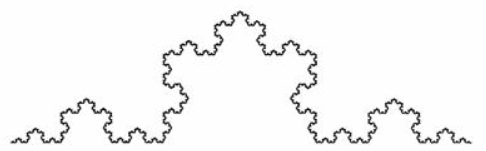
\includegraphics[width=0.75\textwidth]{KochCurve}
		\caption[labelInTOC]{Koch-görbe}
	\end{center}
\end{figure}
\subsection{Implementáció}
A Koch-görbét generáló algoritmus alapja a Line segédosztály. A Line segédosztályban tárolódik minden egyenes két végpontja és hossza. Az osztálynak két fontos metódusa van, az expandLeft és expandRight metódusok. Ezek a metódusok az adott egyenesre rajzolnak háromszöget úgy, hogy a háromszög alapja az egyenes, vagy annak egy bizonyos százaléka, akkor az expandRight metódus adja a háromszög bal oldalát, az expandRight pedig a jobb oldalát.
\begin{lstlisting}
expandLeft(p: any, direction: number, lerp: number, angle: number): Line[] {
	let len = this.length * lerp;
	let alpha = 180 - 2 * p.degrees(angle);
	let sideLength = len * p.sin(angle) / p.sin(p.radians(alpha));
	
	let lerpAmount = (1 - lerp) / 2;
	
	let a = p5.Vector.lerp(this.A, this.B, lerpAmount);
	let dir = p5.Vector.sub(this.B, this.A);
	dir.rotate(-direction * angle);
	let offset = p5.Vector.add(a, dir);
	
	let x = p5.Vector.lerp(a, offset, sideLength / p5.Vector.dist(a, offset));
	
	let newLines = [];
	newLines.push(new Line(this.A, a));
	newLines.push(new Line(a, x));
	
	return newLines;
}
\end{lstlisting}
A metódus paraméterei közé tartozik a direction, ami azt az irányt adja meg, hogy felfelé, vagy lefelé történjen a háromszög oldalának rajzolása, a lerp, ami azt mondja meg, hogy a háromszög alapja hány százaléka az egyenesnek, az angle pedig a háromszög alapja és az oldalai között bezárt szöget adja meg. Ezek a paraméterek a konfigurációs panelben állíthatóak. A függvény kiszámolja a háromszög bal oldalának pontjait, ezekből létrehoz egy új Line objektumot, majd visszaadja egy tömb elemeként. \\
A Koch-görbe konfigurációs lehetőségei a következők:
\begin{itemize}
	\item Gyorsaság
	\item Szín
	\item Vonalvastagság
	\item Vonalhosszúság
	\item Szög
	\item Háromszög alapjának mérete (\%)
	\item Fixált kezdővonal
	\item Irány
	\item Szivárvány mód
\end{itemize}
A fixált kezdővonal opcióval testreszabhatjuk a kezdő egyenes helyét, és méretét, valamint az egér görgőjével rotálhatjuk, majd kattintással elhelyezhetjük a vászonon. A kezdő egyenes megadása esetén az egér mozgására a változások valós időben láthatóak. Kattintáskor az alábbi függvény fut le:
\begin{lstlisting}
p.handleMousePressed = () => {
	if (this.play && !this.useFixedRoot && this.customRoot == null) {
		let center = p.createVector(p.mouseX, p.mouseY);
		let x = p.createVector(p.mouseX - this.length / 2, p.mouseY);
		let y = p.createVector(p.mouseX + this.length / 2, p.mouseY);
		
		let xDir = p5.Vector.sub(x, center);
		xDir.rotate(this.rotation);
		
		let yDir = p5.Vector.sub(y, center);
		yDir.rotate(this.rotation);
		
		let xOffset = p5.Vector.add(center, xDir);
		let yOffset = p5.Vector.add(center, yDir);
		
		this.customRoot = new Line(xOffset, yOffset);
		this.root = this.customRoot;
		this.lines = [this.root];
	}
}
\end{lstlisting}
Egérrel való kattintáskor az egér pozíciója az egyenes közepén van. A függvény ennek a pontnak az x pozíciójához hozzáadja és kivonja belőle az egyenes hosszának felét, az y pozíció mindkét pont esetén változatlan marad, így megkapjuk az egyenes két végpontját. Az így kapott egyenes vízszintes, így ha a felhasználó az egér görgője segítségével rotálta, további számolásokra van szükség. Mindkét végpontból kivonjuk az egyenes középpontját, így két megfelelő irányba mutató vektort kapunk amit a vektorok beépített rotate függvényével könnyen megfelelő pozícióba rotálhatunk. A this.rotation változó tárolja azt az értéket, amennyivel a felhasználó a kezdőegyenest rotálta, ezt az értéket kapja paraméterül ez a függvény. A Koch-görbe draw függvénye hasonló, mint a Sierpinszki-szőnyegé, így ezt nem részletezném.
\section{Levy-C Görbe}
A Lévy C görbét először Enresto Cesàro és Georg Faber írta le és tanulmányozta a differenciálhatóságát, azonban mégis Paul Lévy francia matematikus nevét viseli, aki a fraktál önhasonlóságát definiálta. Ez a fraktál alapjáraton nagyon hasonlít a Koch görbére, egyedüli eltérés, hogy az egyenesekre való háromszögek rajzolásakor nem az egyenes egy bizonyos százalékából lesz a háromszög alapja, hanem a teljes egyenesből. Mivel az algoritmus implementációja és a konfigurációs lehetőségek is nagyon hasonlítanak a Koch görbe alguritmuséhoz, így ezt a fraktált nem részletezem tovább.
\section{Hilbert görbe}
A Hilbert görbe a térkitöltő görbék csoportjába tartozik. Az első térkitöltő görbét ugyan Peano alkotta meg, de Hilbert volt az, aki először érthető
geometriai képet tudott mutatni egy általa definiált térkitöltő görbéről. Megadott egy
geometriai generáló eljárást, amivel létrehozta ezen görbék egy osztályát.
Egy térkitöltő görbét rekurzívan adhatunk meg, bizonyos lépések végtelen sokszori alkalmazásával. A Hilbert görbe első iterációjának megrajzolása úgy történik, hogy veszünk egy egységnégyzetet a következő pontokkal:
\begin{itemize}
	\item (0, 0) pont a négyzet bal alsó sarka
	\item (0, 1) pont a négyzet bal felső sarka
	\item (1, 1) pont a négyzet jobb felső sarka
	\item (1, 0) pont a négyzet jobb alsó sarka
\end{itemize}
Ezt az egységnégyzetet képzeletben további 4 szabályos négyzetre bonjuk, és egy töröttvonalat húzunk, úgy, hogy az átmenjen a mind a négy négyzet középpontján az alábbi sorrendet követve: A bal alsó sarokban levő négyzet középpontjából indul, majd felfelé megy a bal felső négyzet középpontjáig, innen jobbra a jobb felső négyzet középpontjáig, majd a jobb alsó négyzet középpontjában áll meg. Ezzel egy fordított U alakzatot kapunk. 
\begin{figure}[!ht]
	\begin{center}
		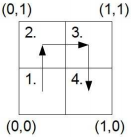
\includegraphics{HilbertCurve1-1}
		\caption[labelInTOC]{Hilbert görbe 1. iterációja}
	\end{center}
\end{figure}
\begin{figure}[!ht]
	\begin{center}
		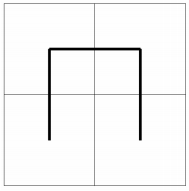
\includegraphics[width=0.5\textwidth]{HilbertCurve1-2}
		\caption[labelInTOC]{Hilbert görbe 1. iterációja}
	\end{center}
\end{figure}
A Hilbert görbe második iterációja 4 egységnégyzetből áll, mindegyikben megrajzolva az első iteráció fordított U alakzatát. A bal alsó négyzetet 90 fokkal jobbra, a jobb alsó négyzetet 90 fokkal balra forgatjuk, így a két alsó U alakzat egymástól "elfelé" néz. Végül az U alakzat megrajzolásával megegyező sorrendben (bal alsó, bal felső, jobb felső, jobb alsó) összekötjük mind a 4 egységnégyzetben levő alakzatok egymáshoz legközelebbre eső végpontjait.
\begin{figure}[!ht]
	\begin{center}
	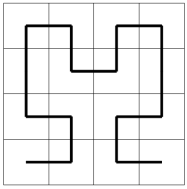
\includegraphics[width=0.5\textwidth]{HilbertCurve2-1}
	\caption[labelInTOC]{Hilbert görbe 2. iterációja}
\end{center}
\end{figure}
\subsection{Implementáció}
Az implementációt úgy kezdtem, hogy kiszámoltam hány négyzetből és hány pontból fog állni a Hilbert görbe. Ehhez a következő egyenlőségeket használtam:\\
$N = 2^I$,
$P = N^2$, ahol N a négyzetek száma, I az iteráció, P pedig a pontok száma. Az iteráció adott, ugyanis a felhasználó konfigurációs lehetőségként meg kell adja, hogy hanyadik iterációig szeretné, hogy az algoritmus fusson. Az algoritmus draw függvénye úgy működik, hogy minden képrfissítéskor eggyel mélyebbre megy a pontok tömbjén, és összeköti az adott pontot a tömbben levő előző ponttal, ezzel egy animációs hatást keltve. Az algoritmus viszonylag kevés konfigurációs lehetőséggel bír, ezek a következők:
\begin{itemize}
	\item Gyorsaság
	\item Vonalvastagság
	\item Iteráció
	\item Szín
	\item Szivárvány mód
\end{itemize}
\section{Pitagorasz-fa}
A Pitagorasz-fa egy négyzetekből álló fraktál, amelyet Albert Bosman fedezett fel. A nevét onnan kapta, hogy minden egymást érintő négyzet hármas egy szabályos háromszöget zár be. Ha a legnagyobb négyzet, L x L méretű (törzs), akkor a teljes Pitagorasz-fa elfér egy 6L x 4L méretű négyzetben. A hagyományos, egyenlő szárú Pitagorasz-fa a következőképpen konstruálható: az első iterációban létrejön a törzse, amely egy négyzet. A második iterációban a törzsnek a felső élére egy egyenlő szárú derékszögű háromszög rajzolunk úgy, hogy átfogója a négyzet felső éle, valamint a háromszög két befogójából kiágazik az első két ág, amelyek szintén négyzetek. Ezután minden iterációban ez ismétlődik, azaz minden korábbi négyzet felső élére egy egyenlő szárú derékszögű háromszög nő, és azok befogói új négyzetágakat növesztenek. Minden négyzet mérete sqrt(2)/2 értékkel skálázódik le a szülő négyzet méretéhez képest.
\begin{figure}[!ht]
	\begin{center}
		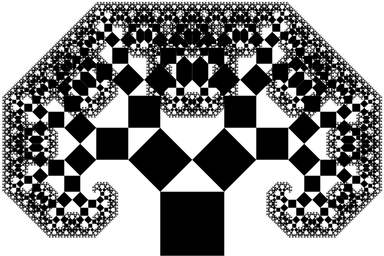
\includegraphics[width=0.5\textwidth]{PythagorasTree}
		\caption[labelInTOC]{Pitagorasz-fa}
	\end{center}
\end{figure}
\subsection{Implementáció}
Az kód átláthatósága érdekében itt is egy segédosztályt írtam először. Ebben az osztályban tárolódnak a négyzetek pontjai illetve mérete. Továbbá, két fontos függvényt tartalmaz, az expandLeft és expandRight függvényeket, amelyek az adott négyzet bal és jobb oldali négyzetágait adják meg. 
\begin{lstlisting}
expandRight(p: any, angle: number): Rectangle {
	let A: p5.Vector;
	let B: p5.Vector;
	let C: p5.Vector;
	let D: p5.Vector = this.B;
	
	let center = p5.Vector.lerp(this.A, this.B, .5);
	let dir = p5.Vector.sub(this.A, center);
	dir.rotate(angle);
	let offset = p5.Vector.add(center, dir);
	
	C = p5.Vector.lerp(center, offset, this.size * 0.5 / p5.Vector.dist(offset, center));
	
	A = p5.Vector.sub(D, C);
	A.rotate(-p.PI/2);
	A = p5.Vector.add(C, A);
	A = p5.Vector.lerp(C, A, 1);
	
	B = p5.Vector.sub(C, D);
	B.rotate(p.PI/2);
	B = p5.Vector.add(D, B);
	B = p5.Vector.lerp(D, B, 1);
	
	let left = new Rectangle(A, B, C, D);
	
	return left;
}
\end{lstlisting}
Az új négyzetek pontjai vektorműveletek sorozatával számolódnak ki. A pontok elnevezése a következő rendszert követi: 
\begin{itemize}
	\item A - bal felső
	\item B - jobb felső
	\item C - bal alsó
	\item D - jobb alsó
\end{itemize}
A jobb oldali négyzetág D pontja megegyezik a szülő négyzet B pontjával. A C pontot úgy kapom meg, hogy a szülő négyzet B pontjából egy vektort hozok létre, amelyből kivonom a szülő négyzet felső élének középpontjából létrehozott vektort, így egy megfelelő irányba mutató vektort kapok, amelyet rotálok egy bizonyos értékkel. A rotálási szöget a függvény paraméterként kapja, ugyanis ez az érték testreszabható a konfigurációs panelben. A maradék A és B pontok már könnyen kiszámolhatóak, ezeket úgy kapom meg, hogy két új vektort hozok létre, egyik a C-ből D-be, másik a D-ből C-be mutat, majd ezeket 90 fokkal rotálom a megfelelő irányba. A függvény visszatérési értékként egy új négyzet objektumot hoz létre a kiszámított pontokból. Az expandLeft függvény hasonlóan működik, csupán a rotálási irányok változnak. \par Az algoritmus konfigurációs lehetőségei a következők:
\begin{itemize}
	\item Gyorsaság
	\item Fixált szög
	\item Fixált gyökér
	\item Oldalhosszúság
	\item Szín
	\item Szivárvány mód
\end{itemize}
Ha a fixált gyökér lehetőséget kikapcsoljuk, akkor tetszőleges helyen helyezhetünk el gyökér négyzetet a vászonon, ezt az egér görgője segítségével rotálhatjuk, illetve az oldalhosszúság opció érékének változtatásával megadhatjuk a méretét. Hasonlóan, a fixált szög lehetőség kikapcsolásával tetszőleges szöggel elhajlíthatjuk a négyzetágakat jobb vagy bal irányba. A szög megadása az egér segítségével történik. Ahhoz, hogy a felhasználóknak érthető legyen a szög megadásának módja, a törzs négyzet felső élének középpontjából egy egyenes indul az egérmutató pozíciója felé. Ennek egyenesnek a hossza az oldalhosszúság felével egyezik meg. Kattintáskor a program kiszámolja az egyenes és a négyzet felső éle között bezárt szöget, és ezt felhasználja a négyzetágak generálásakor.
\section{Fraktál fa}
A fraktál fa egy viszonylag egyszerűen megkonstruálható fraktál, ami a legismertebb fraktálok közé tartozik. Szerkezete nagyon hasonlít a Pitagorasz-fához, annyi különbséggel, hogy négyzetek helyett egyszerű vonalakból tevődik össze. A fraktál fa első iterációjában csak a törzs van, a másodikban a törzsből két ág nő ki egy bizonyos szöget bezárva a törzzsel. Ez a szög tetszőlegesen állítható a konfigurációs panelben. A további iterációkban ez ismétlődik, tehát a már meglévő ágakből új ágak nőnek ki, ez a végtelenségig ismételhető.  
\begin{figure}[!ht]
	\begin{center}
		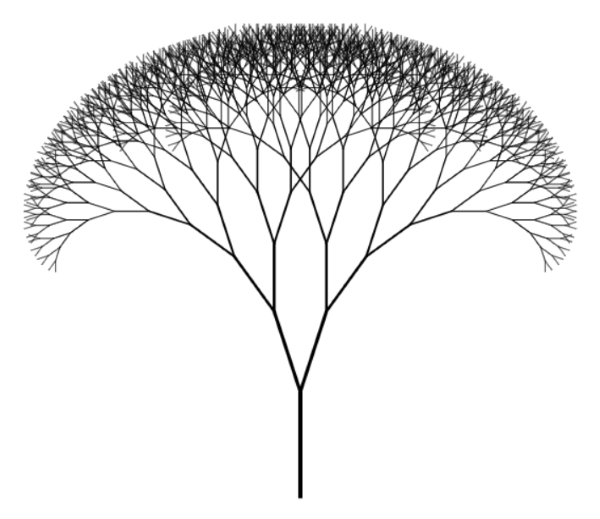
\includegraphics[width=0.5\textwidth]{FractalTree}
		\caption[labelInTOC]{Fraktál fa}
	\end{center}
\end{figure}
\subsection{Implementáció}
A szerkezeti hasonlóságokból eredően az algoritmus implementációja sok helyen hasonlít a Pitagorasz-fáéhoz. Itt is egy segédosztály megírásával kezdtem az implementációt. Ez az osztály tárolja a vonalak A és B végpontjait, valamint hosszát, ezen kívül még tartalmaz egy branch nevezetű függvényt, amely egy adott vonalra meghívva kiszámolja annak az ágait. 
\begin{lstlisting}
branch(p: any, angleLeft: number, angleRight: number, lerpPercentage: number): Line[] {
	let lines: Line[] = [];
	let lerpAmount = this.length * lerpPercentage / this.length;
	
	let dir = p5.Vector.sub(this.A, this.B);
	let xRotated = dir.rotate(angleLeft);
	let xOffset = p5.Vector.add(this.A, xRotated);
	let yRotated = dir.rotate(-angleLeft - angleRight);
	let yOffset = p5.Vector.add(this.A, yRotated);
	let x = p5.Vector.lerp(this.A, xOffset, lerpAmount);
	let y = p5.Vector.lerp(this.A, yOffset, lerpAmount);
	
	lines.push(new Line(x, this.A));
	lines.push(new Line(y, this.A));
	
	return lines;
}
\end{lstlisting}
Ennek a függvénynek 3 fontos paramétere van, az angleLeft, ami megadja a bal oldali ág és a szülő ág által bezárt szöget, az angleRight, ami a jobb oldali ág és a szülő ág által bezárt szöget adja meg, valamint a lerpPercentage, ami azt adja meg, hogy az ágak hossza hány százaléka a szülő ág hosszának. Mivel az egyes vonalak A és B végpontjait vektor típusokként tárolja a segédosztály, ezért az új ágak végpontjai vektorműveletek segítségével könnyen kiszámolhatóak. Az A végpontból kivonva a B végpontot, egy, a vonal irányával megegyező irányú vektort kapok. Ezt, a paraméterben kapott értékekkel jobbra és balra forgatva, megkapom az új ágak A végpontjait. Az új ágak B végpontjai a szülő ág A végpontjával egyeznek meg értelemszerűen. A visszatérési értéke egy tömb, amely az új ágakat tartalmazza.
\par Az algoritmus konfigurációs lehetőségei a következők:
\begin{itemize}
	\item Gyorsaság
	\item Vonalvastagság
	\item Vonalhosszúság
	\item Ágak száma
	\item Elforgatási szög
	\item Ág mérete (\%)
	\item Véletlenszerű szög
	\item Fixált kezdővonal
	\item Szín
	\item Szivárvány mód
\end{itemize}
Az ágak száma opcióval megadható, hogy az egyes ágakból 2 vagy 3 új ág keletkezzen, 3 ág esetén a középső ág iránya megegyezik a szülő ág irányával. A fixált kezdővonal opció kikapcsolásával a fa törzsét adhatjuk meg tetszőlegesen, hasonlóan, mint az előző algoritmusoknál.
\section{H-fa}
A H-fa struktúrája hasonló a Fraktál-fáéhoz. Ez a fraktál merőleges vonalak közvetlen egymás mellé helyezésével konstruálható meg. Minden vonal mindkét végpontján egy rá merőleges vonal halad át, amelynek hossza mindig sqrt(2)-vel kisebb az előző vonal hosszától. Ez egy alapértelmezett érték, ami a konfigurációs panelben tetszőlegesen állítható. A fraktál a nevét onnan kapta, hogy a benne ismétlődő minta a H betűre emlékeztet. A H-fa Hausdorff dimenziója 2.
\begin{figure}[!ht]
	\begin{center}
		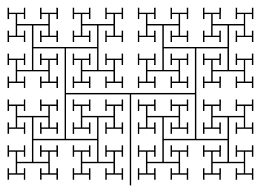
\includegraphics[width=0.5\textwidth]{HTree}
		\caption[labelInTOC]{H-fa}
	\end{center}
\end{figure}
\subsection{Implementáció}
A H-fa egy viszonlyag egyszerűnek mondható fraktál, ezért az implementációja is egyszerű. A függvények, amelyek az ágak pontjainak kiszámolását végzik itt is egy segédosztályban vannak megírva, ezek az expandLeft és expandRight függvények.
\begin{lstlisting}
expandLeft(p: any, lerp: number) {
	let dir = p5.Vector.sub(this.A, this.B);
	dir.rotate(p.PI / 2);
	let xOffset = p5.Vector.add(this.A, dir)
	let x = p5.Vector.lerp(this.A, xOffset, lerp / 2);
	
	dir.rotate(-p.PI);
	let yOffset = p5.Vector.add(this.A, dir);
	let y = p5.Vector.lerp(this.A, yOffset, lerp / 2);
	
	return new Line(x, y);
}
\end{lstlisting}
A segédosztályban a vonalak végpontjai vektorokként vannak tárolva. A végpontokat egymásból kivonva egy vektort kapunk, amelynek iránya megegyezik a vonal irányával, majd ezt jobbra és balra forgatva megkapjuk az bal oldali ág két végpontját. A két új végpontot nem teljesen kötjük össze a szülő vonal bal oldali végpontjával, az új végpontok irányába csak az új ág hosszának a felével megegyező mértékig megyünk, ezzel megkapva az ág megfelelő hosszát. A jobb oldali ág kiszámítása hasonlóan történik.
\par Az algoritmushoz tartozó konfigurációs lehetőségek a következők:
\begin{itemize}
	\item Gyorsaság
	\item Vonalvastagság
	\item Vonalhosszúság
	\item Ág hosszúság (\%)
	\item Fixált kezdővonal
	\item Szín
	\item Szivárvány mód
\end{itemize}